% XeLaTeX 编译
\documentclass[11pt]{article}

\usepackage[final]{acl}

% 标准包
\usepackage{times}
\usepackage{latexsym}
\usepackage[T1]{fontenc}
\usepackage[utf8]{inputenc}
\usepackage{microtype}
\usepackage{inconsolata}
\usepackage{graphicx}
\usepackage{subcaption}
\usepackage{amsmath}
\usepackage{float}
\usepackage{multirow}
\usepackage{booktabs}
\usepackage{url}
\usepackage{xcolor}

% 中文支持
\usepackage{fontspec}
\usepackage{xeCJK}
\setCJKmainfont[BoldFont=STHeiti, ItalicFont=STKaiti]{STSong}
\setCJKsansfont{STHeiti}
\setCJKmonofont{STFangsong}

\definecolor{skyblue}{RGB}{135,206,235}

\title{
\includegraphics[width=0.06\textwidth]{./figs/logo.png} EAGLE-3：通过训练时测试扩展大语言模型的推理加速}

\author{Yuhui Li\textsuperscript{1,3}, Fangyun Wei\textsuperscript{2}, Chao Zhang\textsuperscript{1}, Hongyang Zhang\textsuperscript{3,4}\\
 \textsuperscript{1}北京大学
 \textsuperscript{2}微软研究院 \\
 \textsuperscript{3}滑铁卢大学
 \textsuperscript{4}Vector Institute\\
 \texttt{yuhui.li@stu.pku.edu.cn, fawe@microsoft.com}\\
 \texttt{c.zhang@pku.edu.cn, hongyang.zhang@uwaterloo.ca}
 }

\begin{document}
\maketitle

\begin{abstract}

现代大语言模型（LLM）的顺序生成特性使其推理代价高昂且速度缓慢，而推测性采样（speculative sampling）已被证明是解决该问题的有效方案。EAGLE 等方法在特征层面执行自回归，通过复用目标模型的顶层特征来取得比原始推测性采样更优的效果。LLM 社区中日益兴起的趋势是通过扩大训练数据来提升模型智能，同时不增加推理成本。然而，我们观察到扩大数据规模对 EAGLE 的提升十分有限。我们发现，这一局限源于 EAGLE 的特征预测约束。本文提出 EAGLE-3，它放弃了特征预测，转而直接预测词元（token），并通过名为"训练时测试"的技术，以多层特征融合取代对顶层特征的依赖。这些改进显著提升了性能，使草稿模型能够充分受益于训练数据的扩大。我们的实验涵盖对话模型和推理模型，在五项任务上进行评估。结果表明，EAGLE-3 可实现高达 6.5 倍的加速比，比 EAGLE-2 提升约 1.4 倍。在 SGLang 框架中，EAGLE-3 在批大小为 64 时实现了 1.38 倍的吞吐量提升。代码已开源：\url{https://github.com/SafeAILab/EAGLE}。

\end{abstract}

\begin{figure}
  \begin{subfigure}{\linewidth}
    \centering
    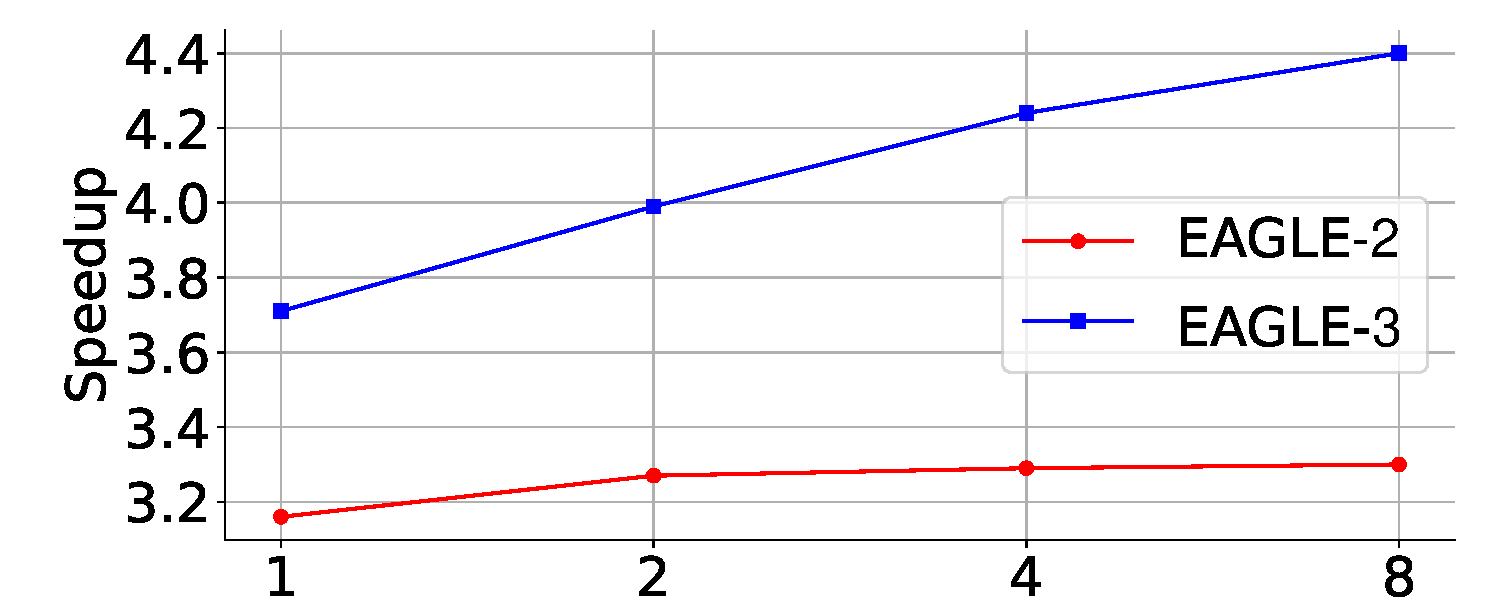
\includegraphics[width=\linewidth]{figs/scaale.pdf}
    \label{fig:sc02}
  \end{subfigure} \hfill
  \begin{subfigure}{\linewidth}
    \centering
    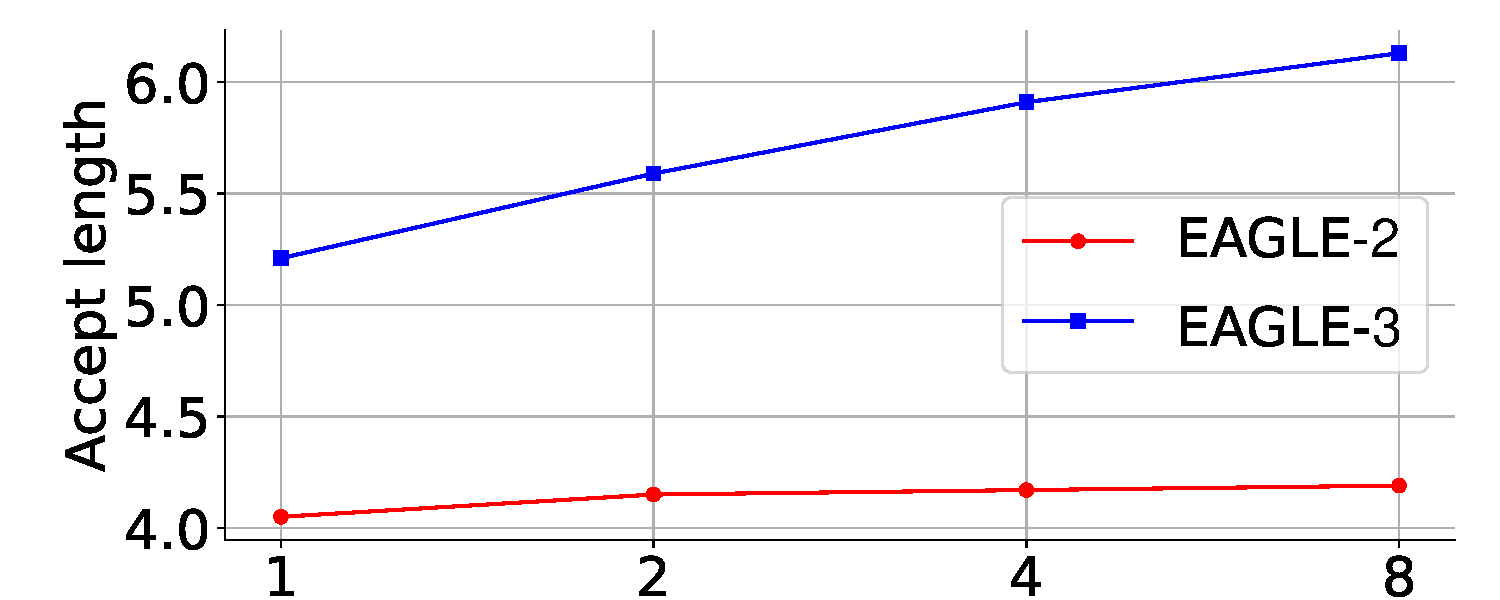
\includegraphics[width=\linewidth]{figs/scaletau.pdf}
    \label{fig:sc03}
  \end{subfigure}
  \vspace{-0.8cm}
  \caption{以 LLaMA-Instruct 3.1 8B 为目标模型在 MT-bench 上评估的扩展规律，横轴为相对于 ShareGPT 的数据规模。EAGLE-3 的新架构设计实现了单调递增的扩展曲线，这在此前的工作中从未观察到。}
  \label{fig:sc}
  \vspace{-0.5cm}
\end{figure}

\section{引言}

\begin{figure*}[t]
\centering
  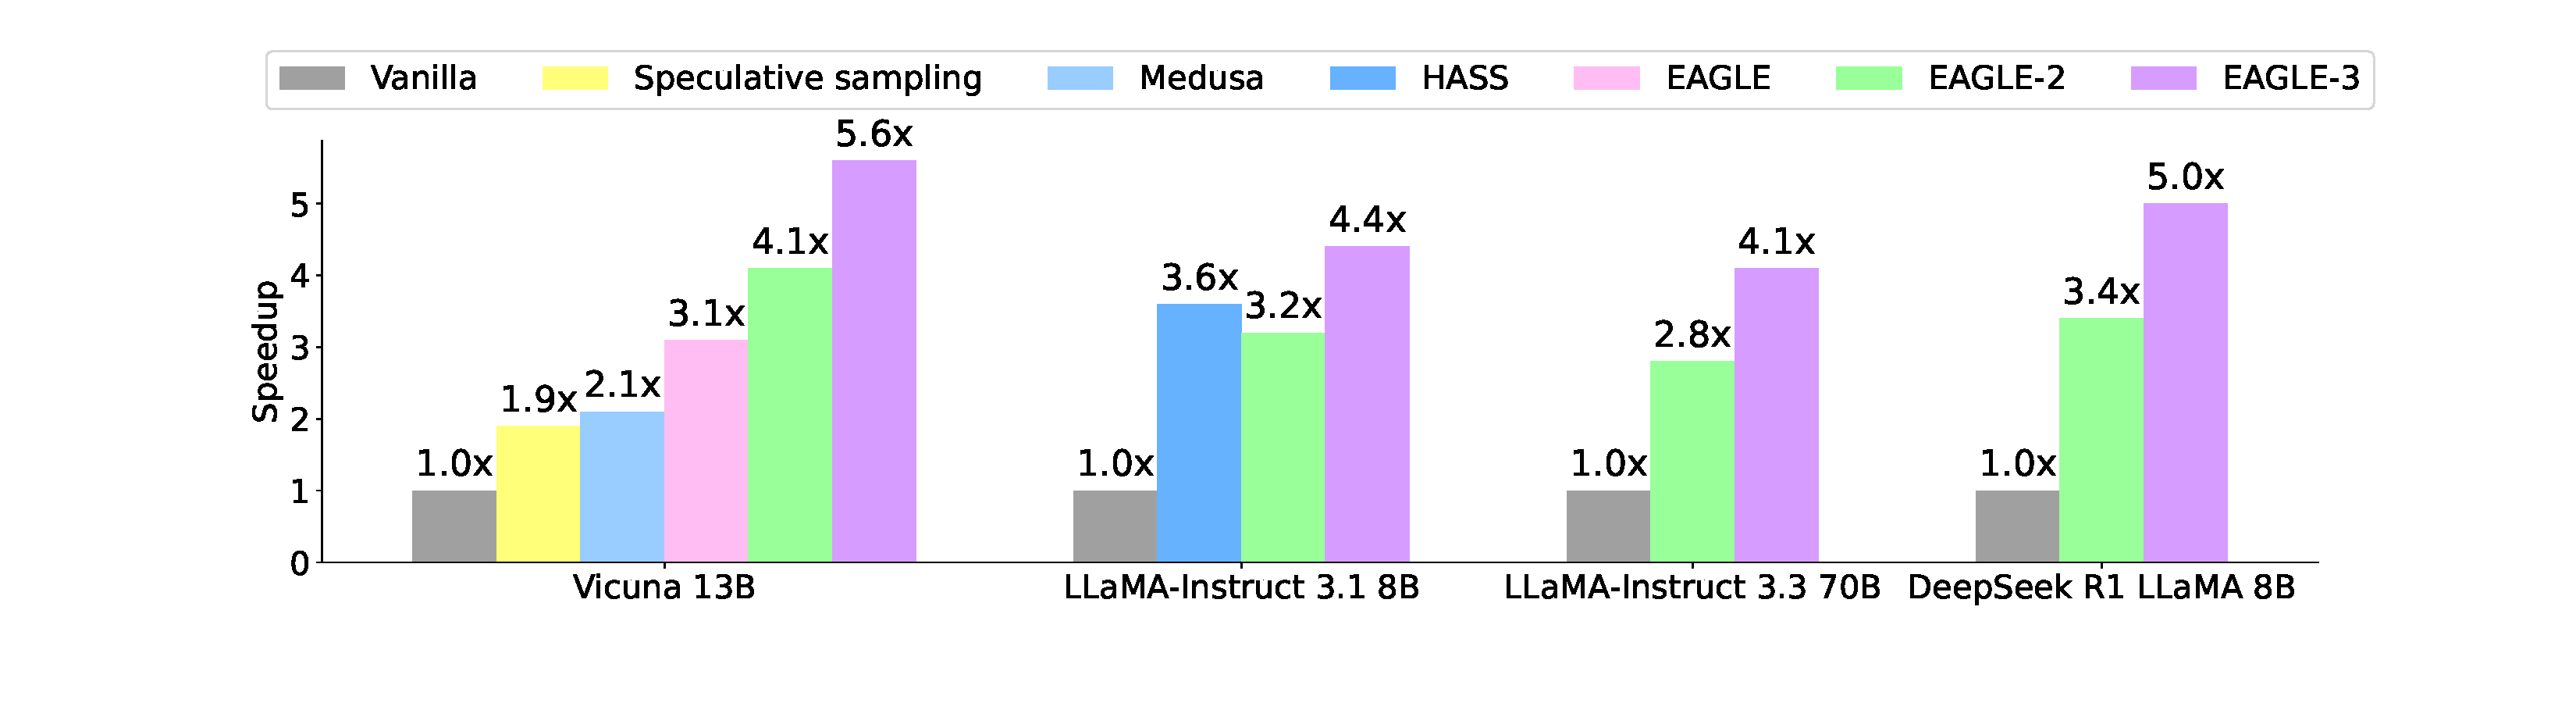
\includegraphics[width=\textwidth]{figs/r1.pdf}
  \vspace{-0.3cm}
  \caption{不同方法在温度=0 时的加速比。对于标准推测性采样，Vicuna-13B 使用 Vicuna-68M 作为草稿模型。表~\ref{tab:experiments} 还提供了与其他方法的对比，但本图仅展示部分方法。对话模型的评测数据集为 MT-bench，推理模型的评测数据集为 GSM8K。DeepSeek R1 LLaMA 8B 指 DeepSeek-R1-Distill-LLaMA 8B。}
  \label{fig:speedup}
  \vspace{-0.3cm}
\end{figure*}

现代大语言模型正被应用于越来越多的领域，其能力的提升主要依赖于模型参数的扩大——部分 LLM 现已超过数千亿参数。在自回归生成过程中，每个词元都需要访问所有模型参数，使得 LLM 推理速度缓慢且成本高昂。

近年来，测试时扩展受到了广泛关注。ChatGPT o1 和 DeepSeek-R1~\cite{guo2025deepseek} 等模型在回答前会进行深思熟虑的推理，以推理时间换取更强的 LLM 能力。然而，这些模型往往需要漫长的推理过程，导致成本极高，而响应时间的增加也严重影响用户体验。推理模型显著提升了推理成本在整个 LLM 流水线中的占比，推动研究者积极探索更廉价、更快速的推理优化方法。

推测性采样方法可通过部分并行化生成过程来降低 LLM 延迟。这些方法快速生成草稿词元，然后并行验证它们，从而在单次前向传播中生成多个词元，显著降低推理延迟。在原始推测性采样中，草稿模型是与目标模型同系列的较小型 LLM，独立运行。与原始推测性采样不同，EAGLE~\cite{li2024eagle} 复用目标模型的顶层特征（LM head 之前的特征），训练草稿模型自回归地预测下一个特征，再利用目标模型的 LM head 获得草稿词元。借助目标模型的丰富信息，EAGLE 相比原始推测性采样取得了更显著的加速效果。HASS~\cite{zhang2024learning} 和 Falcon~\cite{gao2024falcon} 等后续方法也采用了利用当前特征序列预测下一特征的思路。

近期 LLM 越来越依赖更大的训练数据集来提升性能。例如，7B（8B）规模的 LLaMA 系列模型分别使用了 1T、2T 和 15T 词元的训练数据（LLaMA 1~\cite{touvron2023llama}、LLaMA 2~\cite{touvron2023llama2}、LLaMA 3~\cite{dubey2024llama}），在保持模型架构和推理成本基本不变的情况下，各项指标均取得了显著提升。同样地，我们希望通过增加训练数据来提升 EAGLE 的接受率和加速比。遗憾的是，我们观察到额外训练数据对 EAGLE 的收益十分有限。

我们对这一现象的原因进行了分析。如图~\ref{fig:nofe} 上部所示，EAGLE 在特征层面执行自回归预测，预测下一个特征后再输入目标模型的 LM head 获取词元分布。EAGLE 的损失函数包含两个部分：特征预测损失 $l_{\text{fea}}$ 和词元预测损失 $l_{\text{token}}$。得益于特征预测损失，仅在第一步训练的草稿模型可以适应第二步，并获得多步预测能力。然而，以词元预测为最终目标时，特征预测可视为一种额外约束，限制了草稿模型的表达能力，使其难以从更多数据中获益。去除特征约束并扩大训练数据后（图~\ref{fig:nofe} 中部），如图~\ref{fig:sc1} 所示，第一个草稿词元的接受率 $0$-$\alpha$ 显著提升。
然而，草稿模型在第一步输出的 $\hat{a}_{t+1}$ 与真实值 $f_{t+1}$ 相差较大，导致第二步输入序列 $f_1,f_2,\cdots,f_t,\hat{a}_{t+1}$ 偏离训练分布，使第二个草稿词元的接受率 $1$-$\alpha$ 极低，如图~\ref{fig:sc1} 所示。我们可以通过在训练过程中引入第一步（图~\ref{fig:nofe} 下部）来解决这一问题。采用此方法后，增加训练数据的收益更加显著。我们将这一技术命名为\textbf{训练时测试}（training-time test）。

\begin{figure}[t]
  \centering
  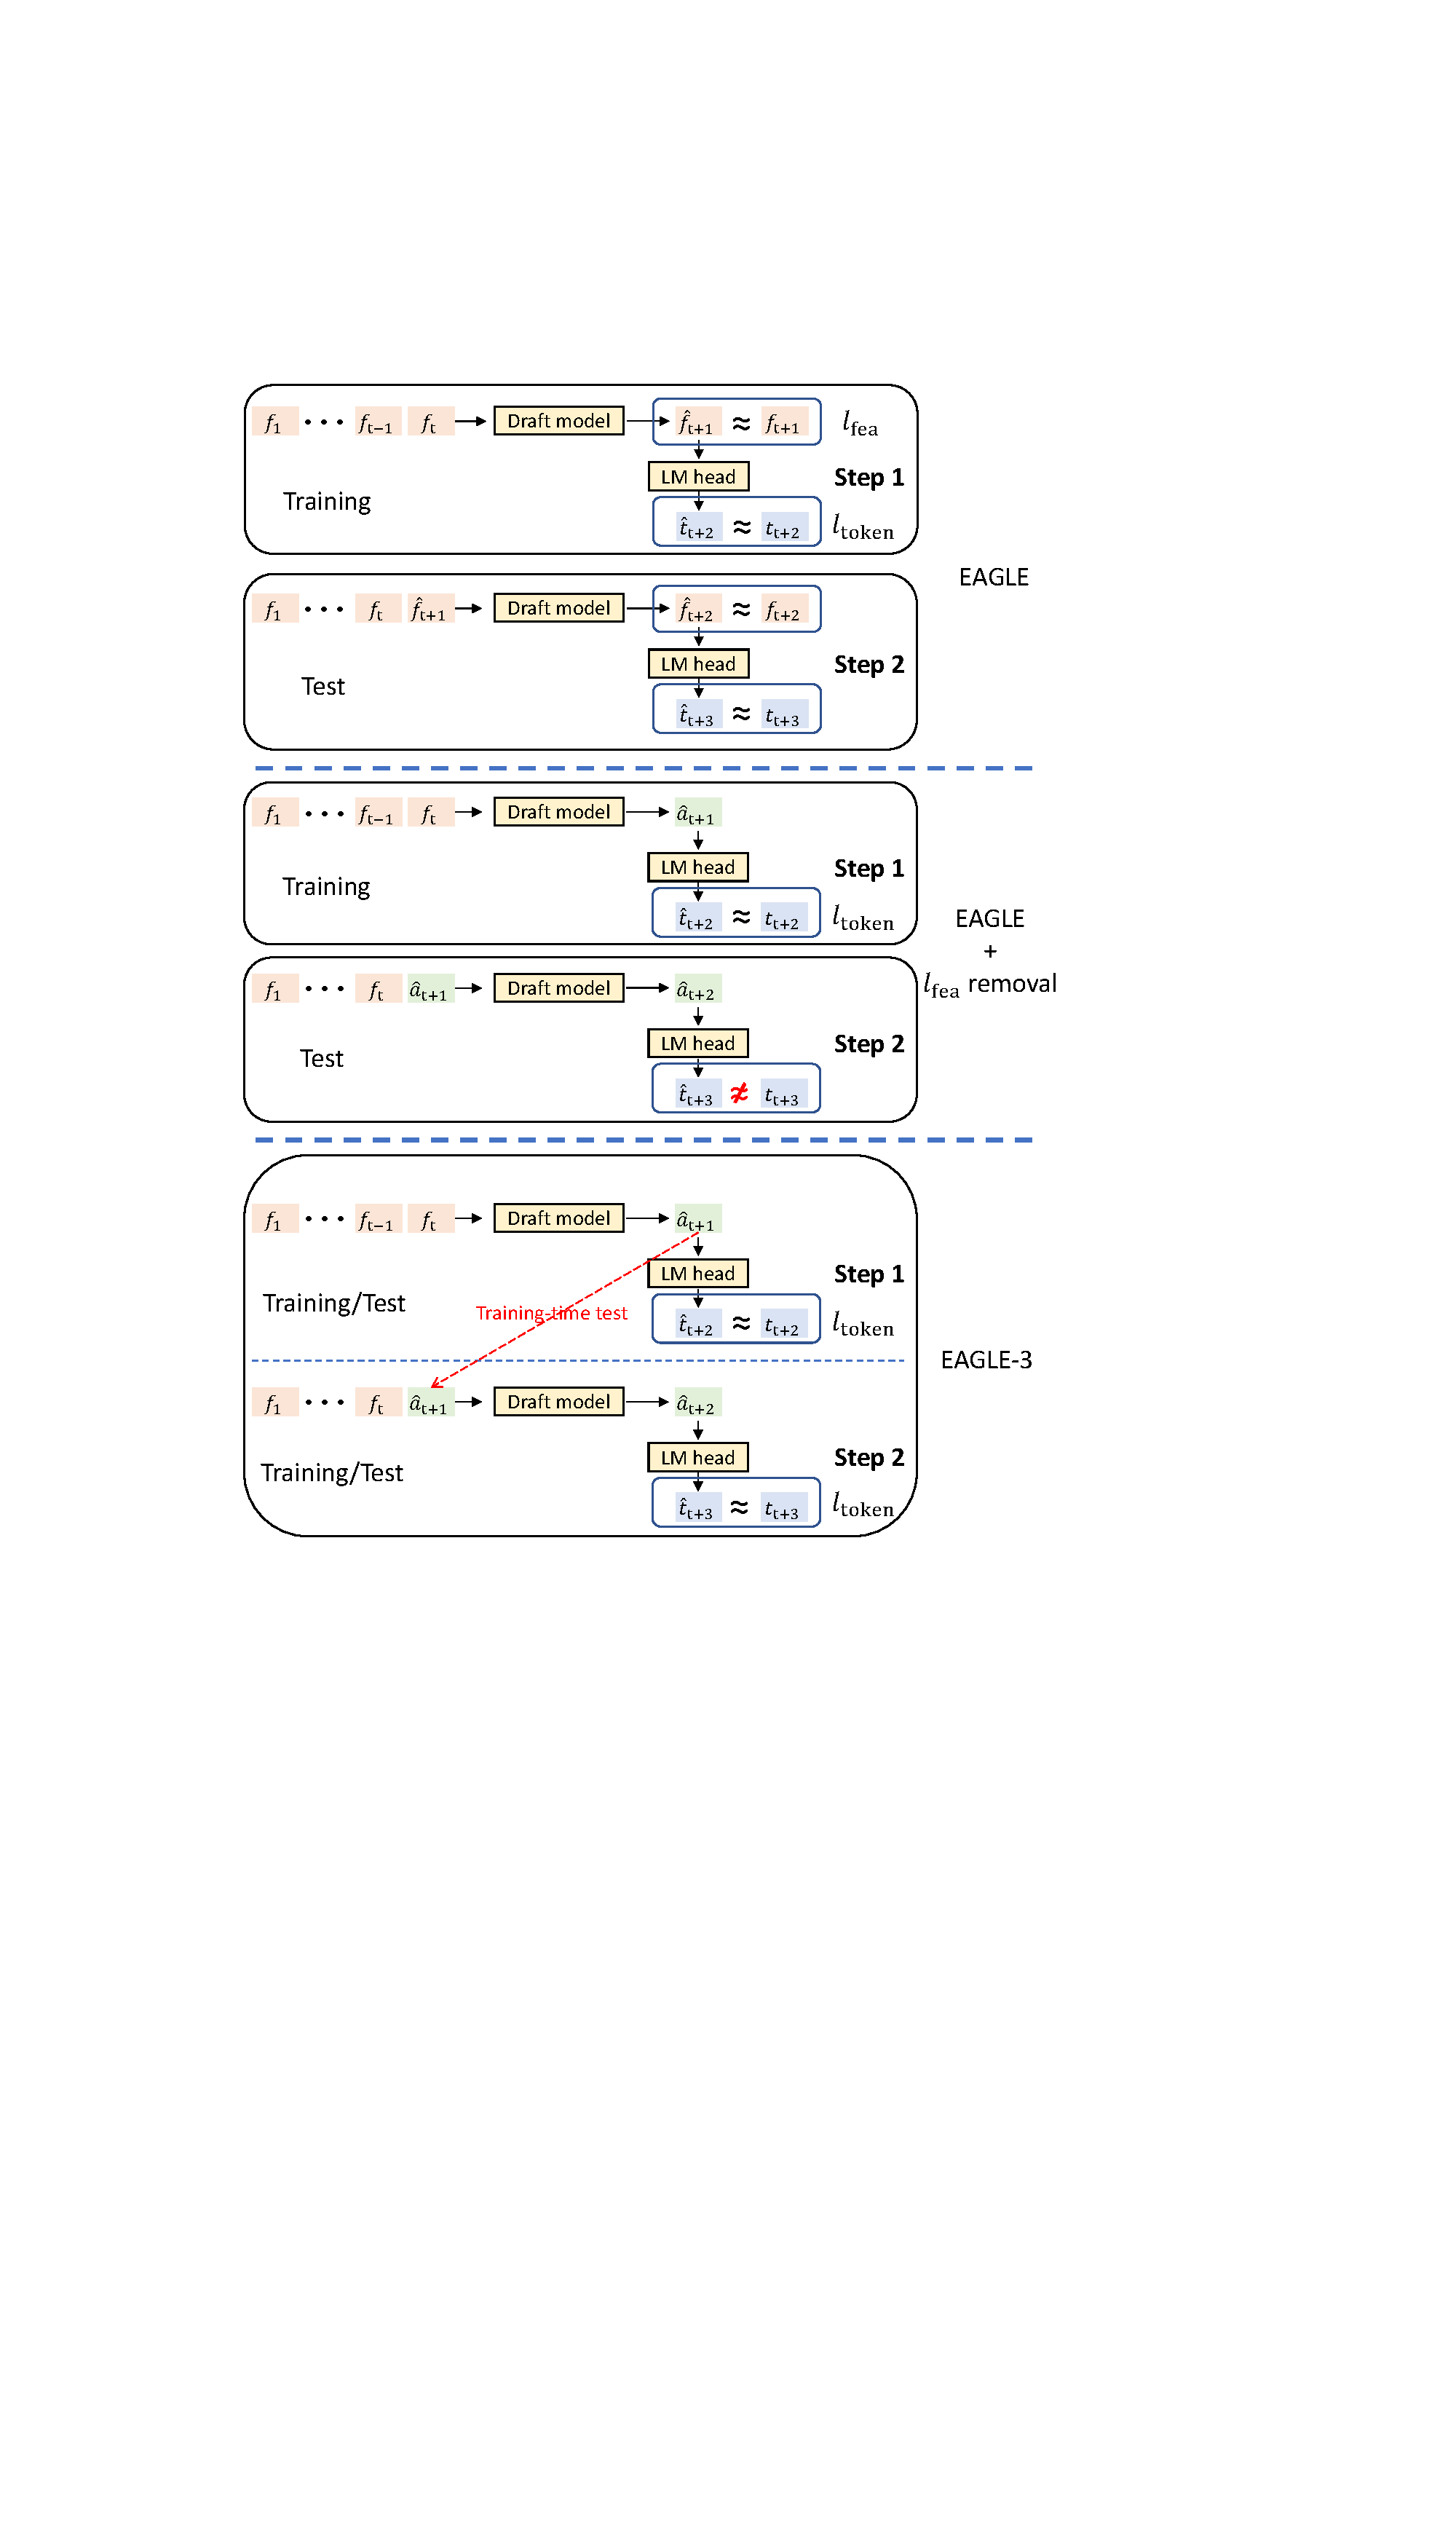
\includegraphics[width=1.07\columnwidth]{figs/nofe.pdf}
  \vspace{-0.5cm}
  \caption{\textbf{训练时测试}（下部）及其与其他草稿方法（上部和中部）的对比示意图。$f$ 表示特征，$t$ 表示词元，$a$ 表示无约束向量。帽符号（hat）表示模型的预测值。图中所有方法均使用前一时间步的词元序列，但为简洁起见未在图中展示。EAGLE-3 的实际输入并非 $f$，详细说明见后续章节。}
  \label{fig:nofe}
  \vspace{-0.5cm}
\end{figure}

\begin{figure}
  \begin{subfigure}{0.49\linewidth}
    \centering
    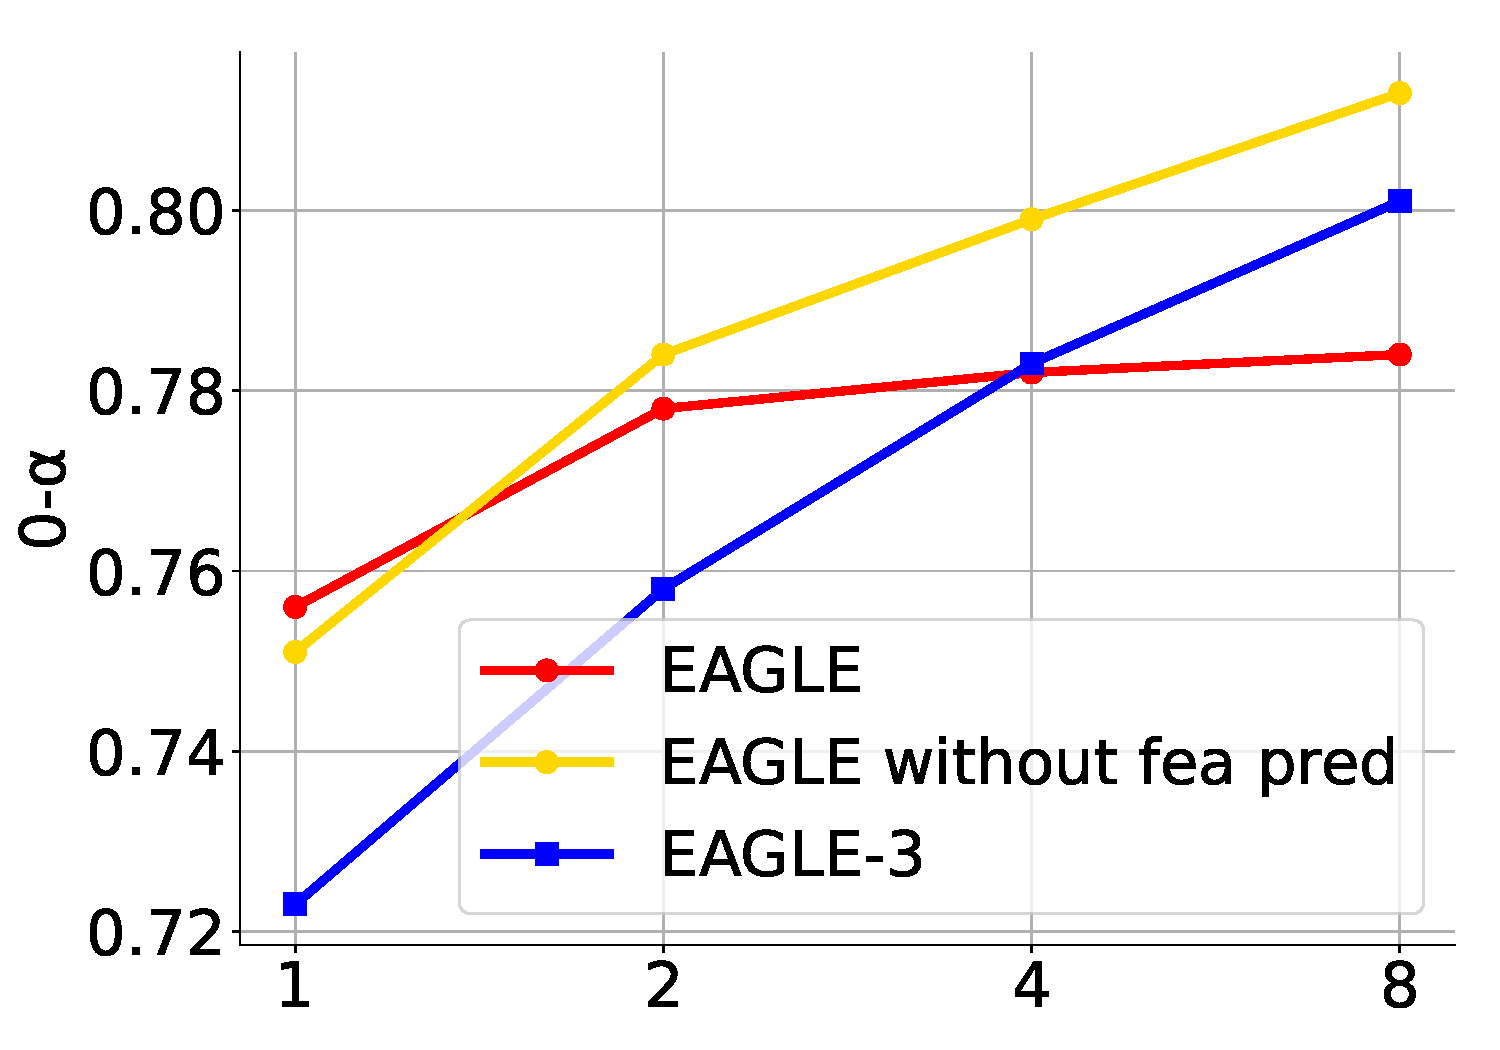
\includegraphics[width=\linewidth]{figs/alpha0.pdf}
    \label{fig:sc00}
  \end{subfigure} \hfill
  \begin{subfigure}{0.49\linewidth}
    \centering
    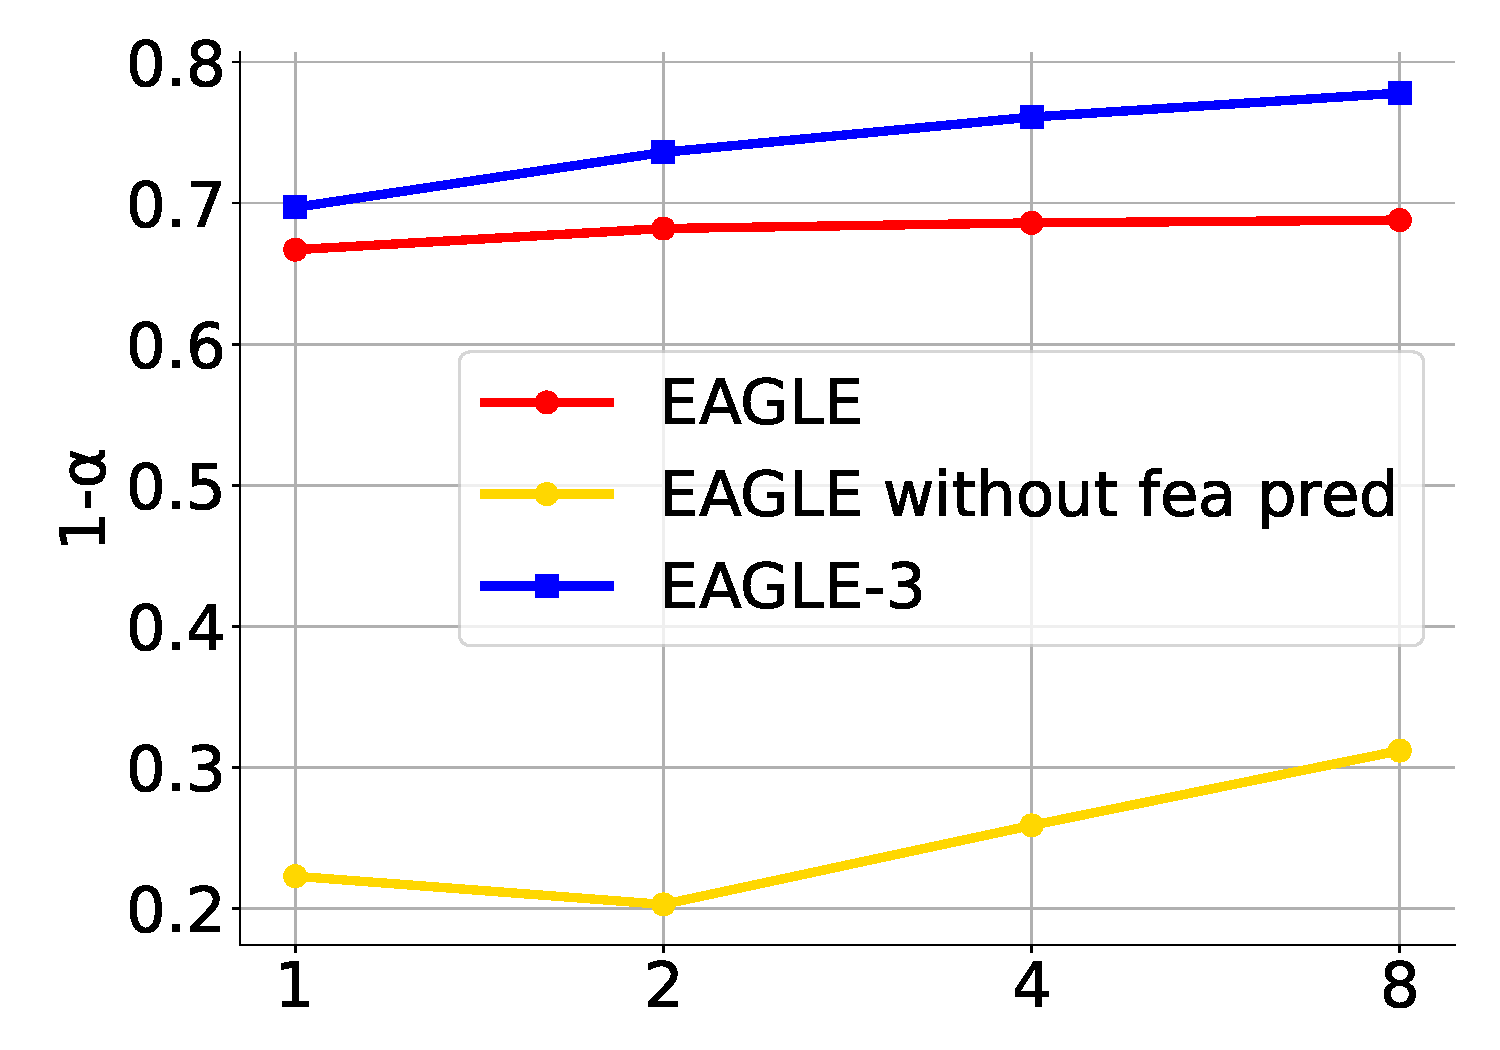
\includegraphics[width=\linewidth]{figs/alpha1.pdf}
    \label{fig:sc01}
  \end{subfigure}
  \caption{不同方法的接受率对比，横轴为相对于 ShareGPT 的数据规模。}
  \label{fig:sc1}
  \vspace{-0.5cm}
\end{figure}

EAGLE 以及 Medusa~\cite{cai2024medusa} 等推测性采样方法复用目标模型的顶层特征，即紧邻 LM head 之前的特征。对于满秩权重矩阵的 LM head，对应下一词元 logits 的顶层特征是唯一的，确保这些特征所含信息与下一词元的 logits 直接对应。然而，仅凭本质上局限于下一词元的顶层特征来预测下下个词元，是一项巨大挑战。幸运的是，上述训练时测试技术使得使用中间层特征成为可能，无需仅依赖顶层——因为训练时已移除特征预测损失 $l_{\text{fea}}$。

综上所述，本文提出 EAGLE-3，即 EAGLE 的增强版本，实现了显著的加速提升。EAGLE-3 支持并行化，并与 EAGLE-2~\cite{li2024eagle2} 的草稿树技术完全兼容。本文的主要贡献如下：
\begin{itemize}
    \item
    \textbf{面向草稿模型的新型训练时测试架构：} 我们去除了特征预测约束，在训练过程中模拟多步生成来直接预测词元。这种直接词元预测方式为草稿模型的输入提供了完全的灵活性。我们不再仅复用顶层特征，而是整合利用目标模型的低层、中层和高层特征，从不同层次捕捉丰富的语义信息。
    \item
    \textbf{发现大语言模型推理加速的扩展规律：} 在新架构下，我们观察到增加草稿模型训练数据量可以同比提升 EAGLE-3 的加速比。这一扩展行为在原始 EAGLE 架构中从未观察到，如图~\ref{fig:sc} 所示。
    \item
    \textbf{更优的推理加速性能：} 使用约 8 倍于 EAGLE 训练数据的 EAGLE-3，在批大小为 1 时实现了比 EAGLE-2 高 1.4 倍的延迟加速。推测性采样常被认为会降低大批大小下的吞吐量。然而，在生产级框架 SGLang~\cite{zheng2024sglang} 中，EAGLE-3 在批大小为 64 时吞吐量提升了 40\%。我们预期更大的数据规模将带来进一步的加速比提升。
\end{itemize}

\section{预备知识}
\subsection{推测性采样}

推测性采样~\cite{leviathan2023fast,chen2023accelerating,sun2024spectr,sun2024optimal} 是一种无损的 LLM 加速技术，交替进行草稿生成和验证，其中草稿生成以低成本进行，验证过程并行化执行。我们用 $t_i$ 表示第 $i$ 个词元，用 $T_{a:b}$ 表示词元序列 $t_a, t_{a+1}, \cdots, t_b$。以 $T_{1:j}$ 作为前缀时，推测性采样的两个阶段如下。

在\textbf{草稿阶段}，推测性采样利用草稿模型（目标模型同系列的较小版本）自回归地生成 $k$ 个词元以构成草稿 $\hat{T}_{j+1:j+k}$，同时记录每个词元的概率 $\hat{p}$。

在\textbf{验证阶段}，推测性采样调用目标模型评估草稿 $\hat{T}_{j+1:j+k}$ 并记录其概率 $p$。推测性采样从前到后依次判断草稿词元是否被接受。对于词元 $\hat{t}_{j+i}$，其被接受的概率为 $\min(1, p_{j+i}(\hat{t}_{j+i})/\hat{p}_{j+i}(\hat{t}_{j+i}))$。若该词元被接受，则继续处理下一个词元；否则，从分布 $\text{norm}(\max(0, p_{j+i} - \hat{p}_{j+i}))$ 中采样一个词元替换 $\hat{t}_{j+i}$，并丢弃草稿中剩余的词元。\cite{leviathan2023fast} 的附录 A.1 证明了推测性采样与原始自回归解码的分布一致性。

\subsection{EAGLE 与 EAGLE-2}

容量有限的草稿模型难以精确逼近大规模目标模型。EAGLE 将目标模型的顶层特征作为额外信息，在特征层面进行自回归，从而简化草稿生成过程。EAGLE 在特征层面执行自回归，再利用目标模型的 LM head 获取草稿词元。由于词元层面的采样结果不可见，特征级自回归引入了不确定性。EAGLE 通过将前一时间步的词元序列（即采样结果）输入草稿模型来解决这一问题。

与原始推测性采样的链式草稿不同，EAGLE 在同一位置生成多个草稿词元，形成树状草稿。在验证阶段，EAGLE 使用树形注意力机制并行验证草稿树。值得一提的是，EAGLE 启发了 DeepSeek-v3~\cite{liu2024deepseek} 预训练中使用的\emph{多词元预测}技术，后者又反过来启发了 EAGLE-3 的新架构设计。

EAGLE~\cite{li2024eagle} 和 Medusa~\cite{cai2024medusa} 等方法使用树形草稿，其草稿树结构是预先定义的、静态的、与上下文无关的。草稿难度与上下文密切相关，静态草稿树可能导致资源浪费。EAGLE-2~\cite{li2024eagle2} 利用草稿模型的置信度近似接受率，并据此动态生成草稿树，在草稿阶段结束时对草稿树进行剪枝。EAGLE-3 同样采用了 EAGLE-2 提出的上下文感知动态草稿树。

\section{EAGLE-3}

本节详细介绍 EAGLE-3 的实现方案。

\subsection{推理流水线}
\label{sec:inf pip}

与其他推测性采样方法一致，EAGLE-3 交替执行草稿生成和验证阶段。EAGLE-3 与 EAGLE 的区别在于草稿阶段，我们通过一个示例加以说明，如图~\ref{fig:pipline} 所示。考虑前缀"How can"（如何能）。

在预填充阶段或上一轮验证阶段中，目标模型执行前向传播，生成下一个词元"I"（我）。我们记录目标模型前向传播中的低层、中层和高层特征序列，分别记为 $l$、$m$ 和 $h$。我们将 $k$ 维向量 $l$、$m$、$h$ 拼接成 $3k$ 维向量，再通过全连接（FC）层降维至 $k$ 维，得到融合了不同层信息的特征 $g$。其中 $k$ 为目标模型的隐藏层维度。

\begin{figure}[t]
  
\includegraphics[width=\columnwidth]{figs/method.pdf}
  \caption{EAGLE-3 推理流水线示意图，展示草稿模型的三个步骤。$l$、$m$、$h$ 分别表示目标模型的低层、中层和高层特征，$e$ 表示词嵌入。}
  \label{fig:pipline}
  \vspace{-0.5cm}
\end{figure}

我们的目标是以"How can I"为前缀生成草稿词元序列。仅输入 $g_\text{how}$ 和 $g_\text{can}$ 时，草稿模型无法访问随机采样过程。因此，类似于 EAGLE~\cite{li2024eagle}，我们引入采样词元"I"的嵌入 $e_\text{I}$。拼接后的向量通过 FC 层降维至 $k$ 维，再输入单层解码器，产生输出 $a$。最后，我们将 $a_\text{I}$ 输入 LM head 并采样得到草稿词元"do"（做）。

在第一步中，以"How can"为前缀，我们复用目标模型的 $g_\text{how}$ 和 $g_\text{can}$。在第二步中，前缀变为"How can I"。理想情况下，我们应复用目标模型的 $g_\text{how}$、$g_\text{can}$ 和 $g_\text{I}$。然而，由于词元"I"尚未经目标模型验证，无法获得 $g_\text{I}$。我们转而使用上一步草稿模型的输出 $a_\text{I}$ 替代 $g_\text{I}$，并将 $a_\text{I}$ 与采样结果"do"的嵌入 $e_\text{do}$ 拼接，作为第一步草稿模型的输入。在第三步中，同样无法获得 $g_\text{do}$，因此使用 $a_\text{do}$ 作为替代，将 $a_\text{do}$ 与 $e_\text{it}$ 拼接作为草稿模型的输入。后续步骤以此类推。

\subsection{草稿模型训练}

\begin{figure*}[t]
  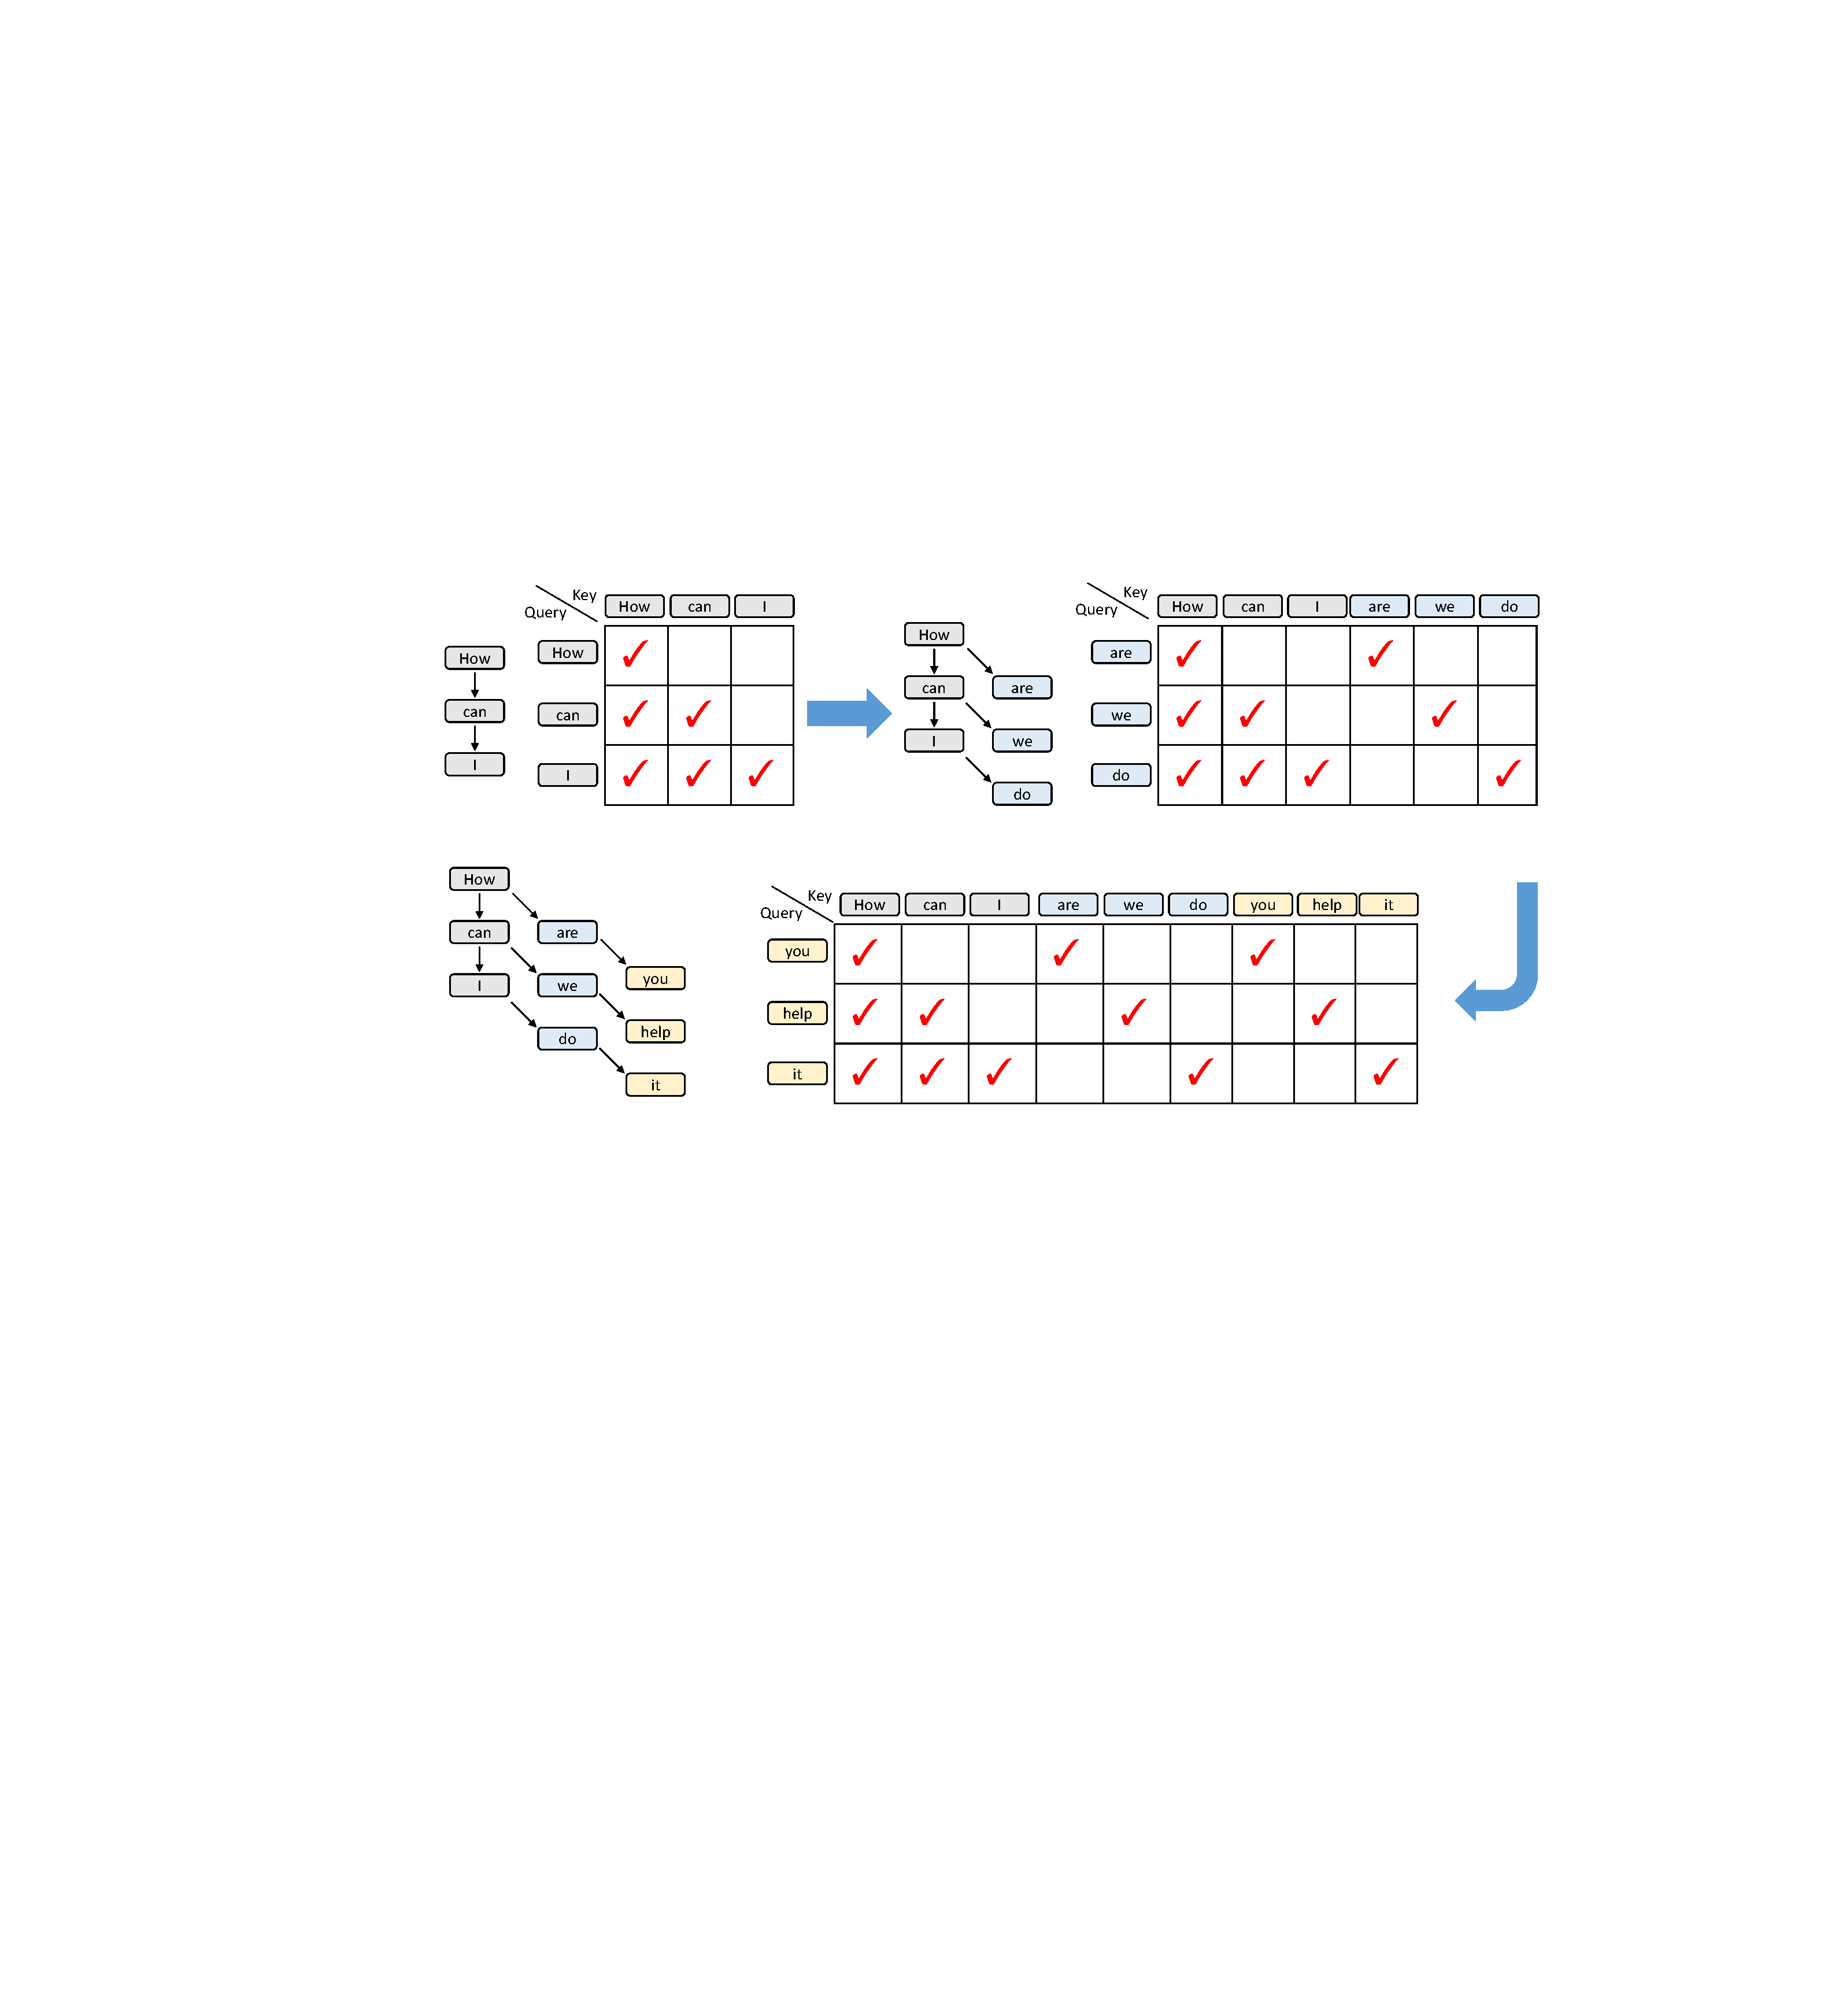
\includegraphics[width=\textwidth]{figs/train.pdf}
  \vspace{-0.5cm}
  \caption{训练时测试中注意力因果掩码的示意图。依次展示一个原生训练步骤（第一步）和两个模拟训练步骤（第二步和第三步）。词元之间的箭头表示上下文关系。\textcolor{gray}{灰色}词元表示训练数据，$\color{skyblue}{\text{蓝色}}$和\textcolor{yellow}{黄色}词元分别表示草稿模型的第一轮和第二轮预测。}
  \label{fig:mask}
\end{figure*}

EAGLE 中草稿模型的输入是，或至少近似于，目标模型的顶层特征 $f_1,f_2,\cdots,f_t$。相比之下，EAGLE-3 中草稿模型的输入既可能是目标模型的特征 $g_1,g_2,\cdots,g_t$，也可能包含草稿模型自身的输出 $a_{t+1},a_{t+2}\cdots,a_{t+j}$。因此，我们需要训练草稿模型以适应不同的输入。在训练过程中，我们执行测试步骤，生成 $a$ 并将其反馈给草稿模型继续训练。

EAGLE-3 草稿模型的核心是一个 Transformer 解码器层。除自注意力操作外，其他组件均不与上下文交互，因此在训练或测试时无需进行其他修改。唯一需要轻微修改的组件是自注意力，下面详细说明。

尽管实际输入为特征，但为便于描述，我们以词元作为输入进行说明。如图~\ref{fig:mask} 所示，原始训练数据是长度为 3 的序列"How can I"，其上下文具有正常的顺序依赖关系，因此注意力掩码为标准下三角矩阵。三个位置的输出分别为"are"、"we"、"do"，它们与"how"、"can"、"I"之间具有树形上下文关系。因此，当输入"are"、"we"、"do"进入第二步时，注意力掩码需要相应调整，如图~\ref{fig:mask} 右上角所示。所有注意力掩码均为对角矩阵，但以原始训练数据为 key 时例外。此时使用矩阵乘法会造成大量计算浪费，因此我们可以通过向量点积仅计算对应位置的注意力分数。

HASS~\cite{zhang2024learning} 和 EAGLE-3 均对注意力机制进行了类似的修改，以在训练中模拟测试过程，但这并非 EAGLE-3 的核心关注点。两者的动机、方法和结果截然不同。HASS 的动机是缓解 EAGLE 中特征预测不准确导致的误差积累。HASS 仍执行特征预测，包含特征预测损失 $l_\text{fea}$，且草稿模型的输入必须是顶层特征。相比之下，EAGLE-3 的动机是去除不必要的约束以增强模型的表达能力。EAGLE-3 不再要求草稿模型的输出拟合目标模型的顶层特征，从而避免了误差积累。去除特征预测损失后，我们还能够发现此前从未被发现的推理加速扩展规律。图~\ref{fig:speedup} 同样展示了 EAGLE-3 和 HASS 的加速效果，EAGLE-3 表现出显著更优的性能。

\section{实验}

\textbf{模型。} 我们在最先进的开源对话和推理模型上进行实验，包括 Vicuna 13B~\cite{vicuna2023}、LLaMA-Instruct 3.1 8B、LLaMA-Instruct 3.3 70B~\cite{dubey2024llama} 和 DeepSeek-R1-Distill-LLaMA 8B~\cite{deepseek2025deepseek}。受 GPU 资源限制，我们无法在 405B 和 671B 模型上测试 EAGLE-3。

\textbf{任务。} 遵循 EAGLE~\cite{li2024eagle} 和 Spec-Bench~\cite{xia2024unlocking} 的设置，我们在五项常见任务上进行评测，对所有任务使用相同权重，不在各任务上微调。多轮对话、代码生成、数学推理、指令遵循和摘要生成分别使用 MT-bench~\cite{zheng2023judging}、HumanEval~\cite{chen2021evaluating}、GSM8K~\cite{cobbe2021training}、Alpaca~\cite{alpaca} 和 CNN/Daily Mail~\cite{nallapati2016abstractive} 数据集。

\begin{table*}[h]
  \centering
  \caption{不同方法的加速比与平均接受长度 $\tau$。V 表示 Vicuna，L31 表示 LLaMA-Instruct 3.1，L33 表示 LLaMA-Instruct 3.3，DSL 表示 DeepSeek-R1-Distill-LLaMA。SpS 表示标准推测性采样，其草稿模型为 Vicuna-68M。Medusa 等方法在非贪心设置下放宽了接受条件，不保证无损加速，因此在温度=1 时不与 EAGLE-3 对比。}
  \resizebox{\linewidth}{!}{
    \begin{tabular}{cccccccccccccc}
    \toprule
          &       & \multicolumn{2}{c}{MT-bench} & \multicolumn{2}{c}{HumanEval} & \multicolumn{2}{c}{GSM8K} & \multicolumn{2}{c}{Alpaca} & \multicolumn{2}{c}{CNN/DM} & \multicolumn{2}{c}{均值} \\
    \midrule
    模型 & 方法 & 加速比 & $\tau$     & 加速比 & $\tau$     & 加速比 & $\tau$     & 加速比 & $\tau$     & 加速比 & $\tau$     & 加速比 & $\tau$ \\
    \midrule
    \multicolumn{14}{c}{温度=0} \\
    \midrule
    \multirow{8}[2]{*}{V 13B} & SpS   & 1.93x & 2.27  & 2.23x & 2.57  & 1.77x & 2.01  & 1.76x & 2.03  & 1.93x & 2.33  & 1.92x & 2.24 \\
          & PLD   & 1.58x & 1.63  & 1.85x & 1.93  & 1.68x & 1.73  & 1.16x & 1.19  & 2.42x & 2.50  & 1.74x & 1.80 \\
          & Medusa & 2.07x & 2.59  & 2.50x & 2.78  & 2.23x & 2.64  & 2.08x & 2.45  & 1.71x & 2.09  & 2.12x & 2.51 \\
          & Lookahead & 1.65x & 1.69  & 1.71x & 1.75  & 1.81x & 1.90  & 1.46x & 1.51  & 1.46x & 1.50  & 1.62x & 1.67 \\
          & Hydra & 2.88x & 3.65  & 3.28x & 3.87  & 2.93x & 3.66  & 2.86x & 3.53  & 2.05x & 2.81  & 2.80x & 3.50 \\
          & EAGLE & 3.07x & 3.98  & 3.58x & 4.39  & 3.08x & 3.97  & 3.03x & 3.95  & 2.49x & 3.52  & 3.05x & 3.96 \\
          & EAGLE-2 & 4.26x & 4.83  & 4.96x & 5.41  & 4.22x & 4.79  & 4.25x & 4.89  & 3.40x & 4.21  & 4.22x & 4.83 \\
          & EAGLE-3 & \textbf{5.58x} & \textbf{6.65} & \textbf{6.47x} & \textbf{7.54} & \textbf{5.32x} & \textbf{6.29} & \textbf{5.16x} & \textbf{6.17} & \textbf{5.01x} & \textbf{6.47} & \textbf{5.51x} & \textbf{6.62} \\
    \midrule
    \multirow{2}[2]{*}{L31 8B} & EAGLE-2 & 3.16x & 4.05  & 3.66x & 4.71  & 3.39x & 4.24  & 3.28x & 4.12  & 2.65x & 3.45  & 3.23x & 4.11 \\
          & EAGLE-3 & \textbf{4.40x} & \textbf{6.13} & \textbf{4.85x} & \textbf{6.74} & \textbf{4.48x} & \textbf{6.23} & \textbf{4.82x} & \textbf{6.70} & \textbf{3.65x} & \textbf{5.34} & \textbf{4.44x} & \textbf{6.23} \\
    \midrule
    \multirow{2}[1]{*}{L33 70B} & EAGLE-2 & 2.83x & 3.67  & 3.12x & 4.09  & 2.83x & 3.69  & 3.03x & 3.92  & 2.44x & 3.55  & 2.85x & 3.78 \\
          & EAGLE-3 & \textbf{4.11x} & \textbf{5.63} & \textbf{4.79x} & \textbf{6.52} & \textbf{4.34x} & \textbf{6.15} & \textbf{4.30x} & \textbf{6.09} & \textbf{3.27x} & \textbf{5.02} & \textbf{4.12x} & \textbf{5.88} \\
    \midrule
    \multirow{2}[1]{*}{DSL 8B} & EAGLE-2 & 2.92x & 3.80  & 3.42x & 4.29  & 3.40x & 4.40  & 3.01x & 3.80  & 3.53x & 3.33  & 3.26x & 3.92 \\
          & EAGLE-3 & \textbf{4.05x} & \textbf{5.58} & \textbf{4.59x} & \textbf{6.38} & \textbf{5.01x} & \textbf{6.93} & \textbf{3.65x} & \textbf{5.37} & \textbf{3.52x} & \textbf{4.92} & \textbf{4.16x} & \textbf{5.84} \\
    \midrule
    \multicolumn{14}{c}{温度=1} \\
    \midrule
    \multirow{4}[2]{*}{V 13B} & SpS   & 1.62x & 1.84  & 1.72x & 1.97  & 1.46x & 1.73  & 1.52x & 1.78  & 1.66x & 1.89  & 1.60x & 1.84 \\
          & EAGLE & 2.32x & 3.20  & 2.65x & 3.63  & 2.57x & 3.60  & 2.45x & 3.57  & 2.23x & 3.26  & 2.44x & 3.45 \\
          & EAGLE-2 & 3.80x & 4.40  & 4.22x & 4.89  & 3.77x & 4.41  & 3.78x & 4.37  & 3.25x & 3.97  & 3.76x & 4.41 \\
          & EAGLE-3 & \textbf{4.57x} & \textbf{5.42} & \textbf{5.15x} & \textbf{6.22} & \textbf{4.71x} & \textbf{5.58} & \textbf{4.49x} & \textbf{5.39} & \textbf{4.33x} & \textbf{5.72} & \textbf{4.65x} & \textbf{5.67} \\
    \midrule
    \multirow{2}[2]{*}{L31 8B} & EAGLE-2 & 2.44x & 3.16  & 3.39x & 4.39  & 2.86x & 3.74  & 2.83x & 3.65  & 2.44x & 3.14  & 2.80x & 3.62 \\
          & EAGLE-3 & \textbf{3.07x} & \textbf{4.24} & \textbf{4.13x} & \textbf{5.82} & \textbf{3.32x} & \textbf{4.59} & \textbf{3.90x} & \textbf{5.56} & \textbf{2.99x} & \textbf{4.39} & \textbf{3.45x} & \textbf{4.92} \\
    \midrule
    \multirow{2}[2]{*}{L33 70B} & EAGLE-2 & 2.73x & 3.51  & 2.89x & 3.81  & 2.52x & 3.36  & 2.77x & 3.73  & 2.32x & 3.27  & 2.65x & 3.54 \\
          & EAGLE-3 & \textbf{3.96x} & \textbf{5.45} & \textbf{4.36x} & \textbf{6.16} & \textbf{4.17x} & \textbf{5.95} & \textbf{4.14x} & \textbf{5.87} & \textbf{3.11x} & \textbf{4.88} & \textbf{3.95x} & \textbf{5.66} \\
    \midrule
    \multirow{2}[2]{*}{DSL 8B} & EAGLE-2 & 2.69x & 3.41  & 3.01x & 3.82  & 3.16x & 4.05  & 2.64x & 3.29  & 2.35x & 3.13  & 2.77x & 3.54 \\
          & EAGLE-3 & \textbf{3.20x} & \textbf{4.49} & \textbf{3.77x} & \textbf{5.28} & \textbf{4.38x} & \textbf{6.10} & \textbf{3.16x} & \textbf{4.30} & \textbf{3.08x} & \textbf{4.27} & \textbf{3.52x} & \textbf{4.89} \\
    \bottomrule
    \end{tabular}%
    }
  \label{tab:experiments}%
\end{table*}%

\textbf{评测指标。} EAGLE-3 不修改目标模型的权重，使用严格的推测性采样接受条件，确保生成质量无损。因此，我们不评估生成质量，而是使用以下指标评估加速性能：

\begin{itemize}
    \item \textbf{加速比：} 相对于原始自回归解码的实际测试加速比。
    \item \textbf{平均接受长度 $\tau$：} 每个草稿-验证循环平均生成的词元数，对应从草稿中被接受的词元数。
    \item \textbf{接受率 $n$-$\alpha$：} 草稿词元被接受的比例，直接反映草稿模型对目标模型的近似程度。遵循 EAGLE 的设置，在测试接受率时使用链式草稿而非树式草稿。EAGLE 存在误差积累问题，即草稿模型的输入可能是其自身的估计值而非目标模型的精确值。因此，EAGLE 用 $n$-$\alpha$ 表示输入包含 $n$ 个估计特征时的接受率（条件为前面的估计词元均被目标模型接受）。换言之，即输入为 $f_1,f_2,\cdots,f_i,\hat{f}_{i+1},\cdots,\hat{f}_{i+n}$ 时的接受率（$f$ 为精确值，$\hat{f}$ 为草稿模型的估计值）。类似地，我们用 $n$-$\alpha$ 表示 EAGLE-3 中输入包含 $n$ 个自预测值 $a$ 时的接受率，即输入为 $g_1,g_2,\cdots,g_i,{a}_{i+1},\cdots,{a}_{i+n}$ 时的接受率（$g$ 为目标模型的融合特征）。
\end{itemize}

\textbf{实现细节。} 我们使用 AdamW 优化器，$(\beta_1,\beta_2)$ 设置为 (0.9, 0.95)，并实施梯度裁剪（裁剪阈值为 0.5）。学习率设为 5e-5。训练数据使用 ShareGPT 和 UltraChat-200K~\cite{ding2023enhancing}，分别包含约 68K 和 464K 条数据。我们调用目标模型生成回复，而非使用固定数据集。对于推理模型 DeepSeek-R1-Distill-LLaMA 8B，我们还使用了 OpenThoughts-114k-math 数据集进行训练。

\textbf{对比方法。} 以原始自回归解码为基线（1.00x）。我们将 EAGLE-3 与近期无损推测性采样方法进行对比，包括标准推测性采样~\cite{leviathan2023fast,chen2023accelerating,gante2023assisted}、PLD~\cite{saxena2023prompt}、Medusa~\cite{cai2024medusa}、Lookahead~\cite{fu2023lookahead}、Hydra~\cite{ankner2024hydra}、HASS~\cite{zhang2024learning}、EAGLE~\cite{li2024eagle} 和 EAGLE-2~\cite{li2024eagle2}。

\subsection{有效性分析}

图~\ref{tab:experiments} 和表~\ref{tab:experiments} 展示了 EAGLE-3 的加速性能。在所有任务和目标模型上，EAGLE-3 均实现了最高的加速比和平均接受长度。EAGLE-3 相比原始自回归生成实现了约 3.0x--6.5x 的加速，比 EAGLE-2 提升了 20\%--40\%。不同任务对草稿模型接受率的影响不同，因此平均接受长度和加速比均与任务相关。由于代码生成任务中存在大量固定模板，草稿生成最为容易，因此 EAGLE-3 在 HumanEval 上表现最佳，加速比高达 6.5x，平均接受长度高达 7.5。DeepSeek-R1-Distill-LLaMA 8B 是个例外，其在数学推理数据集 GSM8K 上的加速比最高。这可能是因为我们使用了 OpenThoughts-114k-math 数据集训练 DeepSeek-R1-Distill-LLaMA 8B 的草稿模型。

图~\ref{fig:alpha} 展示了以 LLaMA-Instruct 3.1 8B 为目标模型时，EAGLE 和 EAGLE-3 在 MT-bench 上的接受率。EAGLE-3 的接受率显著高于 EAGLE。随着草稿模型自身输入增多，EAGLE 的接受率急剧下降，而 EAGLE-3 的接受率几乎保持不变，验证了训练时测试技术的有效性。

\begin{figure}[h]
  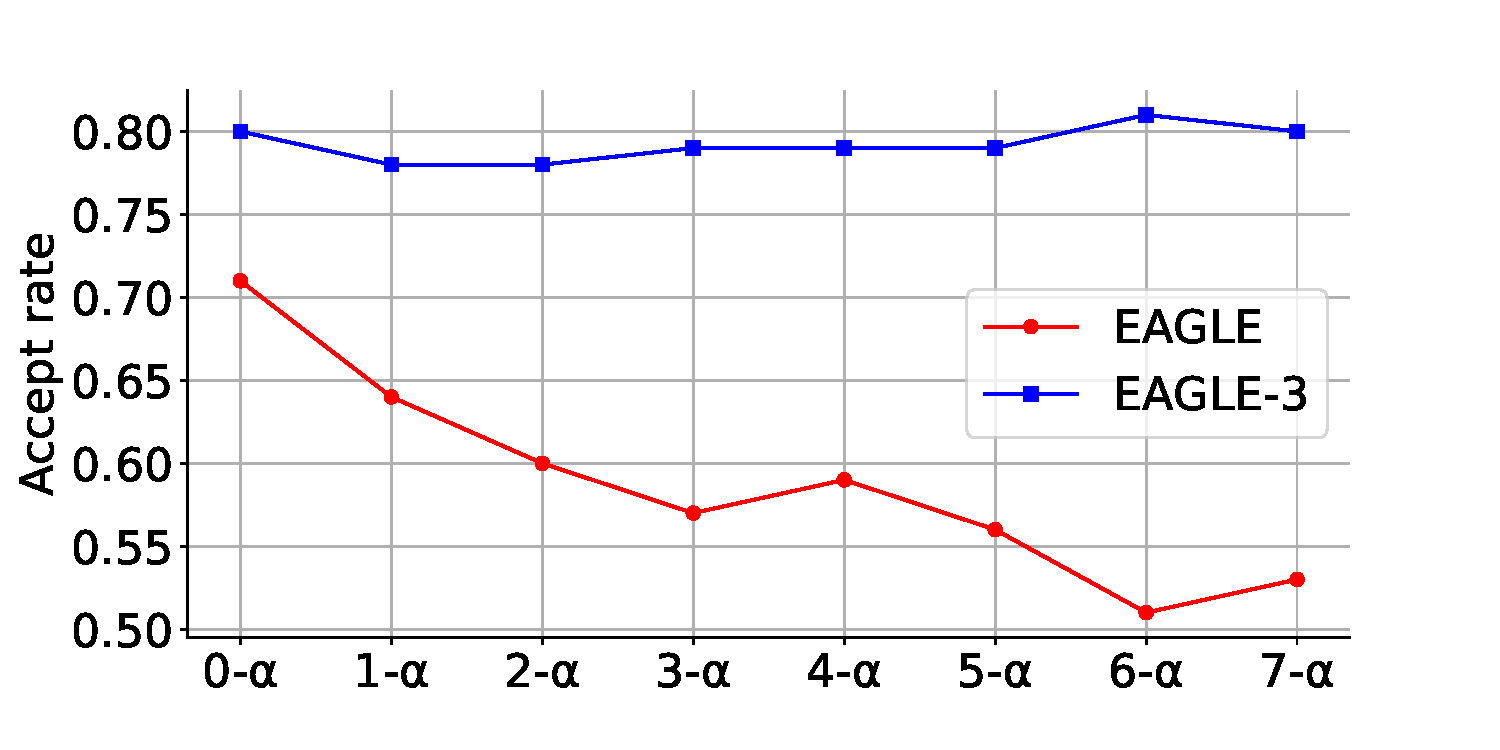
\includegraphics[width=0.95\columnwidth]{figs/alpha.pdf}
  \vspace{-0.2cm}
  \caption{以 LLaMA-Instruct 3.1 8B 为目标模型时，EAGLE 和 EAGLE-3 在 MT-bench 上的接受率。$n$-$\alpha$ 表示在前面的估计词元均被目标模型接受的条件下，输入包含 $n$ 个估计特征时的接受率。}
  \label{fig:alpha}
  \vspace{-0.2cm}
\end{figure}

\subsection{消融实验}

EAGLE-3 的改进主要来自两个方面：第一，去除特征回归约束；第二，将仅复用顶层特征改为复用低层、中层和高层特征的融合。我们以 LLaMA-Instruct 3.1 8B 为目标模型在 MT-bench 上进行了消融实验。结果如表~\ref{tab:aba} 所示，EAGLE-3 的两项改进均显著提升了接受长度和加速比，验证了 EAGLE-3 设计的合理性。

\begin{table}[h]
  \centering
  \caption{以 LLaMA-Instruct 3.1 8B 为目标模型的消融实验结果。"去除特征约束"对应 EAGLE-3 的第一项改进，即去除特征预测约束；"融合特征"对应第二项改进，即以低层、中层和高层特征融合取代顶层特征。}
  \vspace{-0.2cm}
  \resizebox{\linewidth}{!}{
    \begin{tabular}{ccccc}
    \toprule
          & \multicolumn{2}{c}{MT-bench} & \multicolumn{2}{c}{GSM8K} \\
    \midrule
    方法 & 加速比 & $\tau$     & 加速比 & $\tau$ \\
    \midrule
    EAGLE-2 & 3.16x & 4.05  & 3.39x & 4.24 \\
    + 去除特征约束 & 3.82x & 5.37  & 3.77x & 5.22 \\
    + 融合特征（本方法） & 4.40x & 6.13  & 4.48x & 6.23 \\
    \bottomrule
    \end{tabular}%
    }
  \label{tab:aba}%
  \vspace{-0.3cm}
\end{table}%

\subsection{EAGLE-3 在 SGLang 中的表现}

EAGLE-3 等推测性采样算法通过利用冗余计算能力减少内存访问，从而降低内存受限解码阶段的延迟。随着批大小增加，这种冗余减少，推测性采样的效果也随之降低。在高度优化的生产级框架中提升效率更具挑战性。

SGLang 团队在单张 H100 GPU、LLaMA-Instruct 3.1 8B 以及 SGLang v0.4.4 环境~\cite{zheng2024sglang} 下评测了 EAGLE-3 在大批大小时的性能，结果如表~\ref{tab:sglang} 所示。该实验未使用树形结构，链式长度设为 3，测试数据集为 MT-Bench。EAGLE 在批大小为 24 时吞吐量下降，而 EAGLE-3 在批大小为 64 时仍能实现 38\% 的吞吐量提升。

\begin{table}[h]
  \centering
  \caption{在 H100 和 LLaMA-Instruct 3.1 8B 上 MT-Bench 数据集不同批大小下的吞吐量提升，以不使用推测性采样的 SGLang 为基线（1.00x）。实验由 SGLang 团队进行。}
  \resizebox{\linewidth}{!}{
    \begin{tabular}{cccccccccc}
    \toprule
    批大小 & 2     & 4     & 8     & 16    & 24    & 32    & 48    & 56 & 64\\
    \midrule
    EAGLE & 1.40x & 1.38x & 1.23x & 1.02x & 0.93x & 0.94x & 0.88x & 0.99x & 0.99x\\
    EAGLE-3 & 1.81x & 1.82x & 1.62x & 1.48x & 1.39x & 1.32x & 1.38x & 1.34x & 1.38x\\
    \bottomrule
    \end{tabular}%
    }
  \label{tab:sglang}%
\end{table}%

SGLang 团队还测试了在 H100、目标模型为 LLaMA-Instruct 3.1 8B、测试数据集为 MT-bench 时，批大小=1 下 EAGLE-3 的吞吐量，结果如表~\ref{tab:sglang latency} 所示。

\begin{table}[h]
  \centering
  \caption{在 H100、目标模型为 LLaMA-Instruct 3.1 8B、测试数据集为 MT-bench 时批大小=1 下的吞吐量。实验由 SGLang 团队进行。}
  \resizebox{\linewidth}{!}{
    \begin{tabular}{lc}
    \toprule
    方法 & 吞吐量（批大小=1）    \\
    \midrule
    SGLang（无推测性采样，1x H100）& 158.34 词元/秒\\
    SGLang + EAGLE-2（1x H100）& 244.10 词元/秒\\
    SGLang + EAGLE-3（1x H100）& 373.25 词元/秒\\
    \bottomrule
    \end{tabular}%
    }
  \label{tab:sglang latency}%
\end{table}%

\subsection{EAGLE-3 在 vLLM 中的表现}

我们还基于广泛使用的生产级框架 vLLM~\cite{kwon2023efficient}，研究了 EAGLE-3 对大批大小下吞吐量的影响，结果如表~\ref{tab:vllm} 所示（RTX3090，LLaMA-Instruct 3.1 8B）。EAGLE 在批大小为 24 时吞吐量提升最大，而 EAGLE-3 在批大小为 56 时达到最大提升。该实验未使用树形结构，最大链式长度设为 2，测试数据集为 MT-Bench。

\begin{table}[h]
  \centering
  \caption{在 A100 和 LLaMA-Instruct 3.1 8B 上 MT-Bench 数据集不同批大小下的吞吐量提升，以不使用推测性采样的 vLLM 为基线（1.00x）。}
  \resizebox{\linewidth}{!}{
    \begin{tabular}{ccccccccc}
    \toprule
    批大小 & 2     & 4     & 8     & 16    & 24    & 32    & 48    & 56 \\
    \midrule
    EAGLE & 1.30x & 1.25x & 1.21x & 1.10x & 1.03x & 0.93x & 0.82x & 0.71x \\
    EAGLE-3 & 1.75x & 1.68x & 1.58x & 1.49x & 1.42x & 1.36x & 1.21x & 1.01x \\
    \bottomrule
    \end{tabular}%
    }
  \label{tab:vllm}%
\end{table}%

\section{相关工作}

已有许多方法被用于加速 LLM 推理，例如量化~\cite{hubara2018quantized,shen2020q,kim2021bert,zadeh2020gobo,zafrir2019q8bert} 和知识蒸馏~\cite{hinton2015distilling}。这些方法通常存在权衡取舍，需要在模型性能与加速收益之间寻求平衡。

推测性采样使用目标模型进行验证，确保无损加速。早期推测性解码方法~\cite{stern2018blockwise, sun2021instantaneous} 在贪心设置下加速生成，而 \citet{leviathan2023fast, chen2023accelerating} 引入了推测性采样，将草稿-验证框架扩展至非贪心生成。此后涌现出大量改进工作。EAGLE~\cite{li2024eagle}、EAGLE-2~\cite{li2024eagle2}、Medusa~\cite{cai2024medusa} 和 Hydra~\cite{ankner2024hydra} 复用了目标模型的特征。HASS~\cite{zhang2024learning} 在训练过程中模拟多步草稿过程，以缓解 EAGLE 中训练-推理不一致和误差积累问题。GLIDE 和 CAPE~\cite{du2024glide} 复用目标模型的 KV 缓存，而 Draft \& Verify~\cite{zhang2023draft} 等方法~\cite{hooper2023speed,yang2023predictive,monea2023pass,li2024nearest,yi2024generation,liu2024kangaroo,sun2024triforce,elhoushi2024layer,svirschevski2024specexec} 利用层跳过或早退机制复用部分目标模型参数。

\section{结论}

本文提出了 EAGLE-3。在 EAGLE 的基础上，EAGLE-3 包含两项关键改进：第一，去除特征预测约束，通过训练时测试直接预测草稿词元；第二，以目标模型低层、中层和高层特征的融合取代仅使用顶层特征，从而获取更丰富的信息。在这些改进下，EAGLE-3 持续受益于训练数据的增加，实现了高达 6.5 倍的最大加速比。

\section*{致谢}

感谢 James Liu、Ke Bao、Yineng Zhang、Lianmin Zheng、Ying Sheng 以及 SGLang 团队的许多其他成员，感谢他们将 EAGLE-3 合并至 SGLang 环境并进行评测。

\bibliography{custom}

\newpage
\clearpage
\appendix

\section{实现细节}
\label{sec:id}

\textbf{原始方法：} 我们使用 Huggingface Transformers 库中的模型，采用 PyTorch 后端并预分配 KV 缓存。其他方法同样以这些模型为基础。

\textbf{标准推测性采样：} 我们使用 HuggingFace Transformers 库的辅助生成功能。

\textbf{PLD、Lookahead、Medusa 和 Hydra：} 我们使用默认设置和官方发布的权重。

\textbf{EAGLE：} Vicuna 和 LLaMA2-Chat 草稿模型使用官方发布权重，而 LLaMA3-Instruct 使用 ShareGPT 数据集训练（与 Medusa 和 Hydra 保持一致）。

\textbf{EAGLE-2：} 对于 7B（8B）、13B 和 70B 规模的原始 LLM，我们分别将草稿词元总数设为 60、50 和 48，草稿树深度为 6，扩展阶段选择 10 个节点。

\textbf{EAGLE-3：} EAGLE-3 的草稿模型具有显著更高的接受率，使我们能够在保持节点数量与 EAGLE-2 相同的情况下，将草稿树深度从 6 增加到 8。

\end{document}
